%-*-latex-*-
\sectionthree{Heapify-up}
\begin{python0}
from solutions import *; clear()
\end{python0}

The following two operations are the basic tools for min- and maxheaps.

Look at this:

\begin{center}
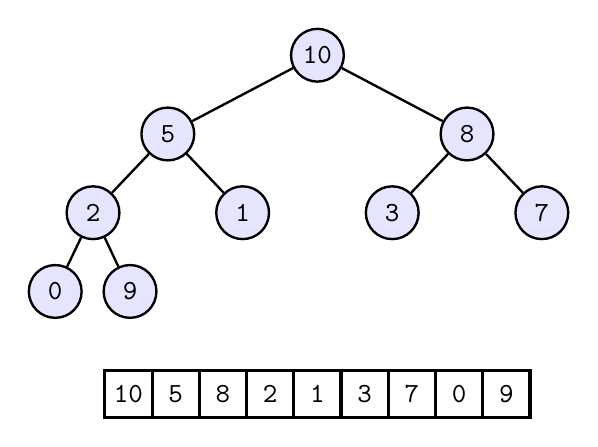
\begin{tikzpicture}

\fill[blue!10] (0.0, 0.0) circle (0.35);
\node [line width=0.03cm,black,minimum size=0.6699999999999999cm,draw,circle] at (0.0,0.0)(10){};\draw (0.0, 0.0) node[color=black] {\texttt{10}};
\fill[blue!10] (-1.9, -1.0) circle (0.35);
\node [line width=0.03cm,black,minimum size=0.6699999999999999cm,draw,circle] at (-1.9,-1.0)(5){};\draw (-1.9, -1.0) node[color=black] {\texttt{5}};
\fill[blue!10] (1.9, -1.0) circle (0.35);
\node [line width=0.03cm,black,minimum size=0.6699999999999999cm,draw,circle] at (1.9,-1.0)(8){};\draw (1.9, -1.0) node[color=black] {\texttt{8}};
\fill[blue!10] (-2.85, -2.0) circle (0.35);
\node [line width=0.03cm,black,minimum size=0.6699999999999999cm,draw,circle] at (-2.85,-2.0)(2){};\draw (-2.85, -2.0) node[color=black] {\texttt{2}};
\fill[blue!10] (-0.95, -2.0) circle (0.35);
\node [line width=0.03cm,black,minimum size=0.6699999999999999cm,draw,circle] at (-0.95,-2.0)(1){};\draw (-0.95, -2.0) node[color=black] {\texttt{1}};
\fill[blue!10] (0.95, -2.0) circle (0.35);
\node [line width=0.03cm,black,minimum size=0.6699999999999999cm,draw,circle] at (0.95,-2.0)(3){};\draw (0.95, -2.0) node[color=black] {\texttt{3}};
\fill[blue!10] (2.85, -2.0) circle (0.35);
\node [line width=0.03cm,black,minimum size=0.6699999999999999cm,draw,circle] at (2.85,-2.0)(7){};\draw (2.85, -2.0) node[color=black] {\texttt{7}};
\fill[blue!10] (-3.33, -3.0) circle (0.35);
\node [line width=0.03cm,black,minimum size=0.6699999999999999cm,draw,circle] at (-3.33,-3.0)(0){};\draw (-3.33, -3.0) node[color=black] {\texttt{0}};
\fill[blue!10] (-2.38, -3.0) circle (0.35);
\node [line width=0.03cm,black,minimum size=0.6699999999999999cm,draw,circle] at (-2.38,-3.0)(9){};\draw (-2.38, -3.0) node[color=black] {\texttt{9}};\draw[line width=0.03cm,black] (10) to  (5);
\draw[line width=0.03cm,black] (10) to  (8);
\draw[line width=0.03cm,black] (5) to  (2);
\draw[line width=0.03cm,black] (5) to  (1);
\draw[line width=0.03cm,black] (8) to  (3);
\draw[line width=0.03cm,black] (8) to  (7);
\draw[line width=0.03cm,black] (2) to  (0);
\draw[line width=0.03cm,black] (2) to  (9);

\draw (-2.3999999999999995, -4.299999999999999)
  node[draw, line width=0.04cm, , color=black,
       rounded corners=0cm, inner sep=0cm] {

\begin{minipage}[t][0.6cm]{0.6cm}
\mbox{}

\end{minipage}

};\draw (-2.3999999999999995, -4.299999999999999) node[color=black] {{\texttt{10}}};
\draw (-1.7999999999999996, -4.299999999999999)
  node[draw, line width=0.04cm, , color=black,
       rounded corners=0cm, inner sep=0cm] {

\begin{minipage}[t][0.6cm]{0.6cm}
\mbox{}

\end{minipage}

};\draw (-1.7999999999999996, -4.299999999999999) node[color=black] {{\texttt{5}}};
\draw (-1.1999999999999997, -4.299999999999999)
  node[draw, line width=0.04cm, , color=black,
       rounded corners=0cm, inner sep=0cm] {

\begin{minipage}[t][0.6cm]{0.6cm}
\mbox{}

\end{minipage}

};\draw (-1.1999999999999997, -4.299999999999999) node[color=black] {{\texttt{8}}};
\draw (-0.5999999999999996, -4.299999999999999)
  node[draw, line width=0.04cm, , color=black,
       rounded corners=0cm, inner sep=0cm] {

\begin{minipage}[t][0.6cm]{0.6cm}
\mbox{}

\end{minipage}

};\draw (-0.5999999999999996, -4.299999999999999) node[color=black] {{\texttt{2}}};
\draw (4.440892098500626e-16, -4.299999999999999)
  node[draw, line width=0.04cm, , color=black,
       rounded corners=0cm, inner sep=0cm] {

\begin{minipage}[t][0.6cm]{0.6cm}
\mbox{}

\end{minipage}

};\draw (4.440892098500626e-16, -4.299999999999999) node[color=black] {{\texttt{1}}};
\draw (0.6000000000000005, -4.299999999999999)
  node[draw, line width=0.04cm, , color=black,
       rounded corners=0cm, inner sep=0cm] {

\begin{minipage}[t][0.6cm]{0.6cm}
\mbox{}

\end{minipage}

};\draw (0.6000000000000005, -4.299999999999999) node[color=black] {{\texttt{3}}};
\draw (1.2000000000000006, -4.299999999999999)
  node[draw, line width=0.04cm, , color=black,
       rounded corners=0cm, inner sep=0cm] {

\begin{minipage}[t][0.6cm]{0.6cm}
\mbox{}

\end{minipage}

};\draw (1.2000000000000006, -4.299999999999999) node[color=black] {{\texttt{7}}};
\draw (1.8000000000000007, -4.299999999999999)
  node[draw, line width=0.04cm, , color=black,
       rounded corners=0cm, inner sep=0cm] {

\begin{minipage}[t][0.6cm]{0.6cm}
\mbox{}

\end{minipage}

};\draw (1.8000000000000007, -4.299999999999999) node[color=black] {{\texttt{0}}};
\draw (2.4000000000000004, -4.299999999999999)
  node[draw, line width=0.04cm, , color=black,
       rounded corners=0cm, inner sep=0cm] {

\begin{minipage}[t][0.6cm]{0.6cm}
\mbox{}

\end{minipage}

};\draw (2.4000000000000004, -4.299999999999999) node[color=black] {{\texttt{9}}};
\end{tikzpicture}

\end{center}



It's almost a maxheap except for the \verb!9!.

What is the simplest way to make it a maxheap?
I compare \verb!9! with it's parent, i.e., \verb!2!.
Since this is a maxheap, something is wrong:
parents should be larger than children.
So I swap \verb!9! and \verb!2! to get:

%-*-latex-*-

\begin{center}
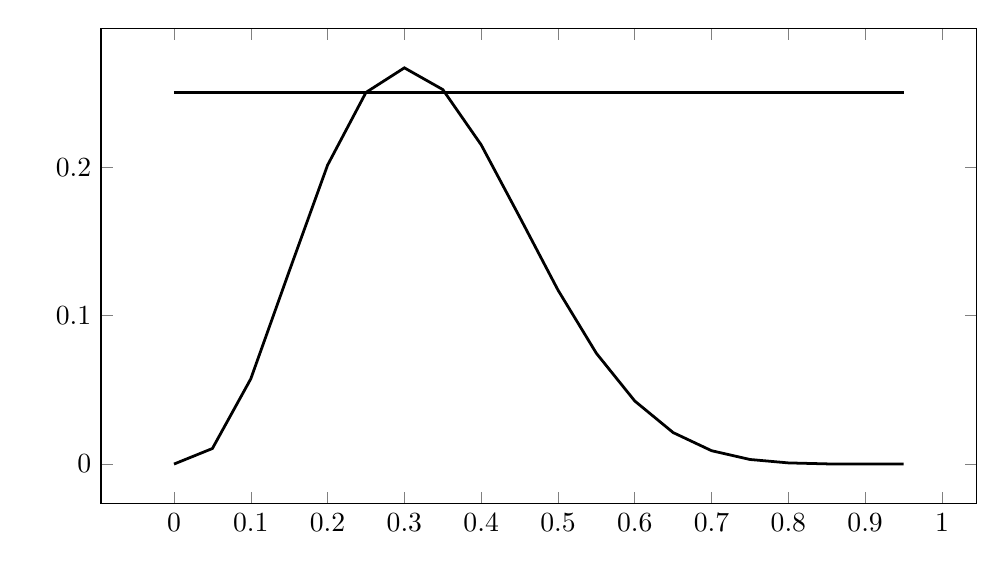
\begin{tikzpicture}[line width=1]
\begin{axis}[width=5in, height=3in,
             scatter/classes={a={mark=*,draw=black}},
             xlabel={\mbox{}},
             xlabel style={name=xlabel}, 
             ylabel={\mbox{}}, 
             legend style={
                at={(xlabel.south)},
                yshift=-1ex,
                anchor=north,
                legend cell align=left,
                },
        ]
]
\addplot[draw=black, line width=1] coordinates {(0.0, 0.0)
(0.05, 0.010475059441406248)
(0.1, 0.05739562800000002)
(0.15, 0.1298337207539062)
(0.2, 0.2013265920000001)
(0.25, 0.25028228759765625)
(0.3, 0.2668279319999998)
(0.35, 0.25221962497265626)
(0.4, 0.21499084799999998)
(0.45, 0.1664782928789064)
(0.5, 0.1171875)
(0.55, 0.07460310631640622)
(0.6, 0.042467328000000006)
(0.65, 0.02120301528515624)
(0.7, 0.009001692000000007)
(0.75, 0.00308990478515625)
(0.8, 0.000786431999999999)
(0.85, 0.0001259148164062501)
(0.9, 8.747999999999988e-06)
(0.95, 8.037890625000049e-08)};\addplot[draw=black, line width=1] coordinates {(0.0, 0.25)
(0.05, 0.25)
(0.1, 0.25)
(0.15, 0.25)
(0.2, 0.25)
(0.25, 0.25)
(0.3, 0.25)
(0.35, 0.25)
(0.4, 0.25)
(0.45, 0.25)
(0.5, 0.25)
(0.55, 0.25)
(0.6, 0.25)
(0.65, 0.25)
(0.7, 0.25)
(0.75, 0.25)
(0.8, 0.25)
(0.85, 0.25)
(0.9, 0.25)
(0.95, 0.25)};
\end{axis}\end{tikzpicture}\end{center}


I then compare \verb!9! and \verb!5! and decide to swap again to get:

%-*-latex-*-

\begin{center}
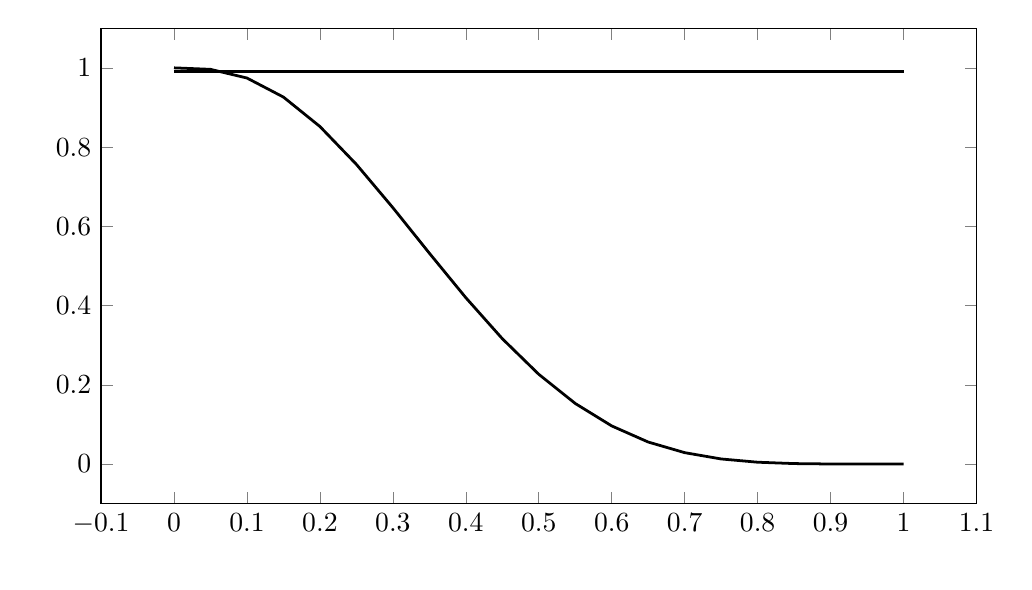
\begin{tikzpicture}[line width=1]
\begin{axis}[width=5in, height=3in,
             scatter/classes={a={mark=*,draw=black}},
             xlabel={\mbox{}},
             xlabel style={name=xlabel}, 
             ylabel={\mbox{}}, 
             legend style={
                at={(xlabel.south)},
                yshift=-1ex,
                anchor=north,
                legend cell align=left,
                },
        ]
]
\addplot[draw=black, line width=1] coordinates {(0.0, 1.0)
(0.05, 0.9962429570312497)
(0.1, 0.9743085000000002)
(0.15, 0.9262348398437498)
(0.2, 0.8519680000000004)
(0.25, 0.75640869140625)
(0.3, 0.6470694999999997)
(0.35, 0.53228332421875)
(0.4, 0.41990399999999994)
(0.45, 0.31644005078125015)
(0.5, 0.2265625)
(0.55, 0.15292768359374995)
(0.6, 0.09625600000000004)
(0.65, 0.055607535156249985)
(0.7, 0.02879550000000002)
(0.75, 0.01287841796875)
(0.8, 0.004671999999999996)
(0.85, 0.0012216445312500006)
(0.9, 0.00017649999999999982)
(0.95, 6.0273437500000275e-06)
(1.0, 0.0)};\addplot[draw=black, line width=1] coordinates {(0.0, 0.99)
(0.05, 0.99)
(0.1, 0.99)
(0.15, 0.99)
(0.2, 0.99)
(0.25, 0.99)
(0.3, 0.99)
(0.35, 0.99)
(0.4, 0.99)
(0.45, 0.99)
(0.5, 0.99)
(0.55, 0.99)
(0.6, 0.99)
(0.65, 0.99)
(0.7, 0.99)
(0.75, 0.99)
(0.8, 0.99)
(0.85, 0.99)
(0.9, 0.99)
(0.95, 0.99)
(1.0, 0.99)};
\end{axis}\end{tikzpicture}\end{center}


Now it's a maxheap.
Basically, you continually swap the value in question with
its parent if the value is larger than the parent.

This is called
\defone{heapify-up}.
It's also called
\defone{bubble up} or
\defone{percolate up}.


In general, if \verb!x[0..n]! is an array
and I can talk about heapify-up on array \verb!x!
treating \verb!x! as a maxheap,
starting at index \verb!i! and going up
along its path to the root (i.e., index 0).

You can also talk about heapify-up on an array
treating it as a minheap,
starting at some index.

For a maxheap, to heapify-up at an index \verb!i!, you compare
\verb!x[i]! and \verb!x[parent(i)]!
and swap them if necessary, i.e. if \verb!x[i]! $>$ \verb!x[parent(i)]!
and you keep following that value up to the root.
If \verb!x[i]! $\leq$ \verb!x[parent(i)]!, you stop.
That's it.

\begin{Verbatim}[frame=single]
ALGORITHM: heapify-up (for maxheap)
INPUTS: x[0..n-1] -- array
        i         -- index of x

while 1:
    if parent(i) < 0: break
    if x[i] > x[parent(i)]:
        swap x[i], x[parent(i)]
        i = parent(i)
\end{Verbatim}

With a tiny of optimization:
\begin{Verbatim}[frame=single]
ALGORITHM: heapify-up (for maxheap)
INPUTS: x[0..n-1] -- array
        i         -- index of x

v = x[i]
while 1:
    p = parent(i)
    if p < 0: break
    if v <= x[p]:
        x[i] = v
        break
    else:
        x[i] = x[p]
        i = p
\end{Verbatim}

The same idea works for minheap.
